\subsection{Разработка клиентской составляющей комплекса}

\subsubsection{Создание нового React-приложения}

Для начала разработки нового React-приложения предпочтительным способом является использование утилиты npx, поставляемой вместе с пакетом Node, с указанием модуля <<create-react-app>> (CRA), который создаёт в указанной директории новое React-приложение с рекомендуемой файловой структурой и со всеми необходимыми зависимостями. При необходимости можно использовать шаблоны, добавляющие дополнительные надстройки React-прило\-жения. Например, для создания приложения с настроенной поддержкой TypeScript можно использовать следующую команду:

\begin{lstlisting}[style=ES6, language=bash]
  npx create-react-app my-app --template typescript
\end{lstlisting}

где my-app является названием нового приложения.

Результат выполнения этой команды представлен на рисунке~\ref{img:cre__init}.

\begin{figure}[H]
  \centering
  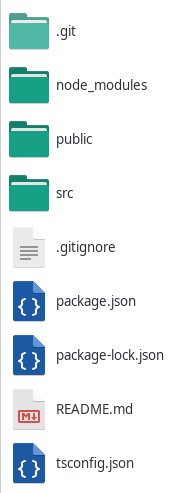
\includegraphics[height=0.3\textheight]{assets/images/practical/cra__init.png}
  \caption{Результат выполнения CRA}
  \label{img:cre__init}
\end{figure}

Папка public содержит содержит файлы описания сайта, такие как сам файл сайта (index.html), логотипы сайта трёх размеров для разных устройств, файл манифеста и файл информации для поисковиков (robots.txt). В index.html в теге body генерируется два элемента:

\begin{enumerate}
  \item <<noscript>> -- отображается, если в браузере отсутствует поддержка JavaScript.
  \item <<div>> -- является входной точкой React приложения в HTML. Внутри этого элемента будут отображены все компоненты приложения.
\end{enumerate}

В папке src основными файлами являются index.tsx, являющийся точкой входа React приложения, а также App.tsx, являющийся основным компонентом, к которому в последствие будут добавляться остальные компоненты приложения.

Для улучшения структуризации приложения, внутри папки src были созданы директории components, containers, providers, routes, styles,  types, в которых расположены файлы соответственно компонентов, страниц, предоставителей контекста, ссылок на компоненты, общих стилей и типов данных. В результате была получена структура, которая представлена на рисунке~\ref{img:cre__struct}.

\begin{figure}[H]
  \centering
  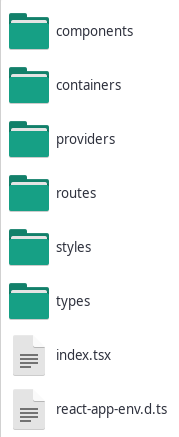
\includegraphics[height=0.3\textheight]{assets/images/practical/cra__struct.png}
  \caption{Структура src CRA}
  \label{img:cre__struct}
\end{figure}

\subsubsection{Разделение приложения на контейнеры}

Веб-приложение делится на две основные части:

\begin{enumerate}
  \item Панель навигации сайта.
  \item Основное наполнение сайта.
\end{enumerate}

Для этого было принято решение использовать модель позиционирования flex, так как эти два основных компонента находятся в одной оси -- вертикальной. В листинге~\ref{lst:site__app} представлен контейнер App приложения.

\lstinputlisting[style=ES6, caption={Контейнер App}, label={lst:site__app}, consecutivenumbers=true]{assets/listings/practical/Client/src/containers/App/App__pract.tsx}

В панели навигации также использовалась модель flex. На панели навигации расположены логотип с названием сайта, а также три кнопки, при нажатии на которые отображается соответствующая страница.

Для отображения необходимой страницы в зависимости от URL, был разработан компонент Main, в котором, для предоставления контекста используется компонент WebSocketProvider, а также компонент Switch, с помощью которого происходит определение, какая страница должна быть отображена для текущего запроса, и отображает необходимую страницу. В листинге~\ref{lst:site__main} представлен компонент Main.

\lstinputlisting[style=ES6, caption={Компонент Main}, label={lst:site__main}, consecutivenumbers=true]{assets/listings/practical/Client/src/components/Main/Main__pract.tsx}

\subsubsection{Разработанное React-приложение}

В ходе разработки веб-приложения были реализованы домашняя страница, на которой выводится состояние комплекса, страница управления светодиодной лентой, страница описания сайта, а также страница, отображающаяся при недействительном адресе. В листинге~\ref{lst:site__home} представлен контейнер домашней страницы.

\lstinputlisting[style=ES6, caption={Контейнер домашней страницы}, label={lst:site__home}, consecutivenumbers=true]{assets/listings/practical/Client/src/containers/HomePage/HomePage__pract.tsx}

В результате разработки веб-приложения был реализован сайт, с помощью которого можно взаимодействовать с комплексом управления светодиодными лентами. Итоговый внешний вид сайта представлен на рисунках~\ref{img:site__about}-\ref{img:site__not-valid}.

\begin{figure}[H]
  \centering
  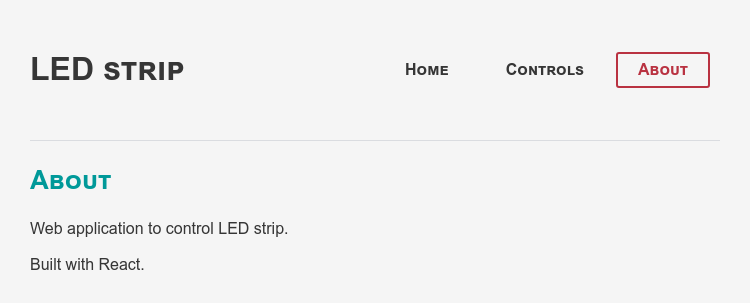
\includegraphics[height=0.2\textheight]{assets/images/practical/site__about.png}
  \caption{Страница описания сайта}
  \label{img:site__about}
\end{figure}

\begin{figure}[H]
  \centering
  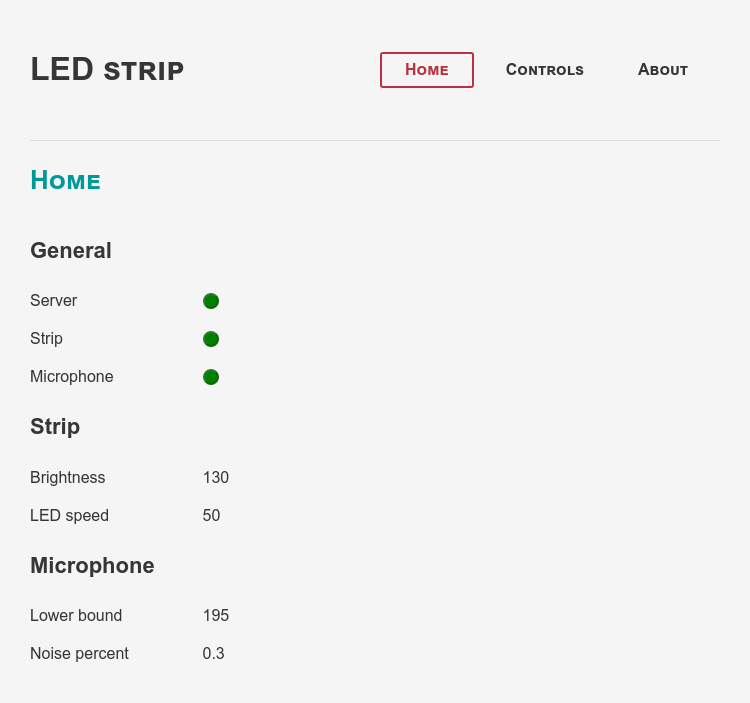
\includegraphics[height=0.4\textheight]{assets/images/practical/site__home.png}
  \caption{Домашняя страница сайта}
  \label{img:site__home}
\end{figure}

\begin{figure}[H]
  \centering
  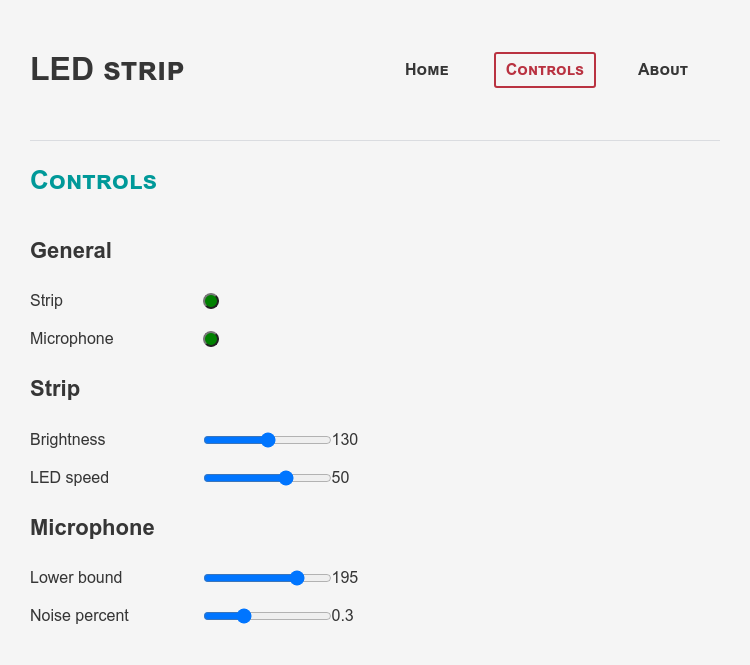
\includegraphics[height=0.4\textheight]{assets/images/practical/site__controls.png}
  \caption{Страница управления комплексом}
  \label{img:site__controls}
\end{figure}

\begin{figure}[H]
  \centering
  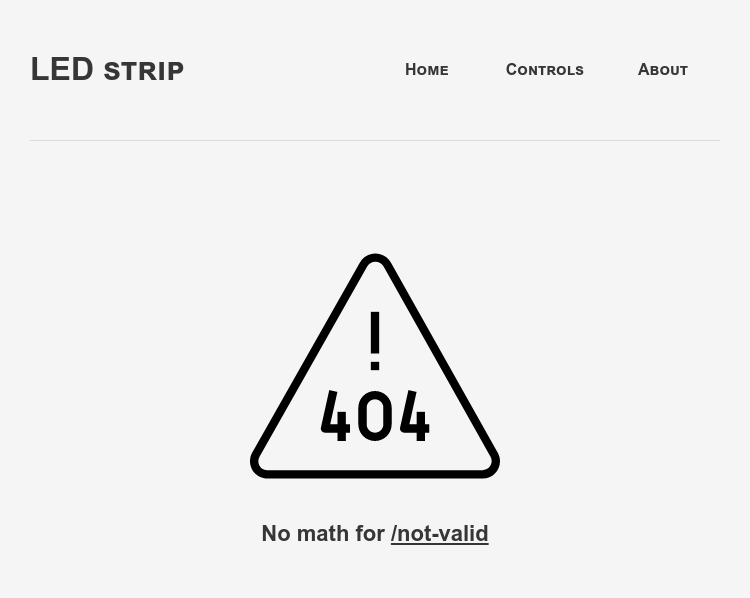
\includegraphics[height=0.4\textheight]{assets/images/practical/site__not-valid.png}
  \caption{Страница, отображающаяся при недействительном адресе}
  \label{img:site__not-valid}
\end{figure}

Полный проект клиентской составляющей комплекса приведён в приложенном к выпускной квалификационной работе DVD-диске.
